\documentclass[aspectratio=169,usenames,dvipsnames]{beamer}
%  \documentclass[usenames,dvipsnames,handout]{beamer}

\usetheme{AnnArbor}
% \usecolortheme{default}
% \usecolortheme{crane}
\usecolortheme{beaver}
\usecolortheme{dolphin}
% \usecolortheme{orchid}
% \usecolortheme{rose}


\usepackage{fourier}
\usepackage{faktor}
\usepackage{amssymb}
\usepackage{amsmath}
\usepackage{amsthm}
\usepackage{faktor}
%\usepackage{stmaryrd}
\usepackage{hyperref}
\usepackage[all]{xy}
\usepackage{tikz}
%    \usetikzlibrary{mindmap,shadows,shapes.geometric,shapes.misc,positioning}
\usepackage{tikz-cd}
% \tikzset{
%     invisible/.style={opacity=0},
%     visible on/.style={alt={#1{}{invisible}}},
%     alt/.code args={<#1>#2#3}{%
%       \alt<#1>{\pgfkeysalso{#2}}{\pgfkeysalso{#3}}%
%   }
% }
%\usetikzlibrary{matrix}
%\usetikzlibrary{calc,intersections}
%\newcommand{\downmapsto}{\rotatebox[origin=c]{-90}{$\large\mapsto$}\mkern2mu} %MnSymbol doesn't work well with beamer
\usepackage{multirow}
% \usepackage{pdfpages}

\def\Q{\mathbb{Q}}
\def\Z{\mathbb{Z}}
\def\C{\mathbb{C}}
\def\R{\mathbb{R}}
\def\F{\mathbb{F}}

\DeclareMathOperator{\AV}{AV}
\DeclareMathOperator{\Mat}{Mat}
\DeclareMathOperator{\Pol}{Pol}
\DeclareMathOperator{\Char}{char}
\DeclareMathOperator{\rk}{Rank}
\DeclareMathOperator{\Frob}{Frob}
\DeclareMathOperator{\ICM}{ICM}
\DeclareMathOperator{\Pic}{Pic}
\DeclareMathOperator{\Aut}{Aut}
\DeclareMathOperator{\Hom}{Hom}
\DeclareMathOperator{\End}{End}
\DeclareMathOperator{\Gal}{Gal}
\DeclareMathOperator{\mSpec}{mSpec}
\DeclareMathOperator{\GL}{GL}
\DeclareMathOperator{\Tr}{Tr}
\DeclareMathOperator{\Jac}{Jac}
%\renewcommand{\char}{char} %CRASHES WITH beamer


\newcommand{\cG}{\mathcal{G}}
%\newcommand{\cB}{{\mathcal B}}
%\newcommand{\cC}{{\mathcal C}}
\newcommand{\cO}{{\mathcal O}}
\newcommand{\cH}{{\mathcal H}}
\newcommand{\cL}{{\mathcal L}}
\newcommand{\cM}{{\mathcal M}}
\newcommand{\cQ}{{\mathcal Q}}
\newcommand{\cT}{{\mathcal T}}
%\newcommand{\cW}{{\mathcal W}}


\newcommand{\vphi}{\varphi}

\newcommand{\p}{{\mathfrak p}}
\newcommand{\frf}{{\mathfrak f}}

\newcommand{\set}[1]{\left\lbrace#1\right\rbrace }
\newcommand{\Span}[1]{\left<#1\right>}

%\newcommand{\AVord}[1]{\AV^{\text{ord}}({#1})}
%\newcommand{\Modord}[1]{\cM^{\text{ord}}({#1})}

%\newcommand{\AVcs}[1]{\AV^{\text{cs}}({#1})}
%\newcommand{\Modcs}[1]{\cM^{\text{cs}}({#1})}

\newcommand{\Acan}{\mathcal{A}_{\mathrm{can}}}
\newcommand{\AcanC}{A_{\mathrm{can}}}
\newcommand{\Palpha}[2]{\mathcal{P}^{\alpha}_{{#1}}({#2})}
\newcommand{\Pone}[2]{\mathcal{P}^{1}_{{#1}}({#2})}

\newcommand{\red}[1]{\textcolor{red}{#1}}
\newcommand{\blue}[1]{\textcolor{blue}{#1}}
\newcommand{\green}[1]{\textcolor{ForestGreen}{#1}}

\newtheorem{df}{Definition}[section]
\newtheorem{remark}[df]{Remark}
\newtheorem{prop}[df]{Proposition}
\newtheorem{cor}[df]{Corollary}



%AUTHOR DETAILS
%%%%%%%%%%%%%%%%%%%%%%%%%%%%%%%%%%%%%%%%%%%%%%%%
\title[ANTS XVI - MIT]{Modules over orders,\\conjugacy classes of integral matrices and\\ abelian varieties over finite fields}
\subtitle{}
\author[Stefano Marseglia]{Stefano Marseglia}
\institute[UPF]{University of French Polynesia}
\date[July 18 2024]{July 18 2024 - ANTS XVI - MIT}

\begin{document}
\begin{frame}{}
   \maketitle
   % \begin{center}
   %    \pause Don't forget to motivate your answers.\\
   %    \pause The use of the (Magma) calculator is allowed.
   % \end{center}
\end{frame}

\begin{frame}{}
   \begin{columns}
      \begin{column}{0.5\textwidth}
         {\Huge Thank you} 
\includegraphics[scale=0.5]{ants.PNG}
      \end{column}
      \pause
      \begin{column}{0.5\textwidth}  %%<--- here
          \begin{center}
            Back in Bristol\dots during the RUMP session\vspace*{2em}
            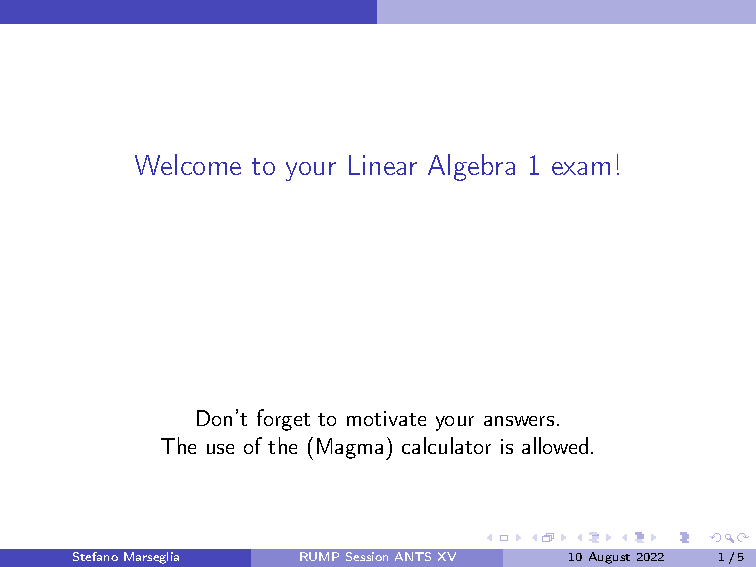
\includegraphics[scale=0.5]{back_in_Bristol.pdf}
           \end{center}
      \end{column}
   \end{columns}
\end{frame}

\begin{frame}{}
   \begin{itemize}
      \item Let $R$ be a commutative ring with unity.
      \item $A,B \in \Mat_{n\times n}(R)$ are {\bf $R$-conjugate} ($A\sim_R B$) if $AP=PB$ for some $P\in \GL_n(R)$.
      \item The {\bf minimal} polynomial $m(x)$ of $A \in \Mat_{n\times n}(R)$ is the polynomial of smallest degree such that $m(A) = O$ (the zero $n\times n$ matrix).
      \item The {\bf characteristic} polynomial of $A \in \Mat_{n\times n}(R)$ is $\det(xI_n-A)$.
   \end{itemize}
   \pause 
   {\bf Question 1:} 
   Are the following two matrices $\Q$-conjugate? Are they $\Z$-conjugate?
   \[
   A=\begin{pmatrix}
      0 & -1 \\ 5 & 0
   \end{pmatrix}, \quad
   B=\begin{pmatrix}
      -1 & 2 \\ -3 & 1
   \end{pmatrix}
   \]
   \pause
   {\bf Answer(s):}\\ 
   \pause Over $\Q$: yes! Same characteristic polynomial $x^2+5$, which is irreducible.\\
   \pause {\bf But...}\\    
   \pause Over $\Z$: no! Why?
\end{frame}

\begin{frame}{}
   {\bf Set-up} 
   Fix monic polynomials $m=m_1\cdots m_n$ and $h=m_1^{s_1}\cdots m_n^{s_n}$ in $\Z[x]$ with 
   \begin{itemize}
      \item each $m_i$ irreducible and 
      \item $m_i\neq m_j$ if $i\neq j$. (i.e.~$m$ is squarefree)
   \end{itemize}
   
   \pause {\bf Question 2}
   Can we describe the representatives of the $\Z$-conjugacy classes of matrices with:
   \begin{itemize}
      \item minimal polynomial $m$, and
      \item characteristic polynomial $h$?
   \end{itemize}
   \pause
   {\bf Answer:}
   \begin{theorem}[(generalized) Latimer-MacDuffee]
      The order $\Z[\pi]=\frac{\Z[x]}{(m)}$ acts on $V=\left(\frac{\Q[x]}{m_1}\right)^{s_1}
      \times \ldots \times 
      \left(\frac{\Q[x]}{m_n}\right)^{s_n}$.\\
      We have a bijection
      \[ \begin{array}{cc}
         \faktor{\set{\parbox[p]{7.5em}{$\Z[\pi]$-lattices in $V$}}}
         {\simeq_{\Z[\pi]}}\\
         \pause \updownarrow\\
         \faktor{\set{\text{matrices with min.~poly.~$m$ and char.~poly.~$h$}}}{\sim_\Z}\\
      \end{array} \]
   \end{theorem}
\end{frame}

\begin{frame}
   \begin{exampleblock}{Example}
      If $h=x^2+5$ then $K=V=\Q(\sqrt{-5})$.\\ 
      The conjugacy classes of matrices with char.~poly $h$ are in bijection with $\Pic(\cO_K)$, which has $2$ elements.
   \end{exampleblock}

   \pause
   Proof (idea):\\
   \begin{itemize}
      \pause
      \item Let $M$ be a $\Z[\pi]$-lattice in $V$ and fix a $\Z$-basis $\mathcal{B}$.
      \pause
      \item Let $A$ be the matrix representing the multiplication-by-$\pi$ wrt $\mathcal{B}$.
      \pause
      \item The induced map is well-defined and injective.
      \pause
      \item For the 'surjectivity' part: take the $\Z$-span of 'algebraic eigenvectors'.
   \end{itemize}
\end{frame}

\begin{frame}{}\
   \newline What about abelian varieties?\\
   \pause
   {\bf Question 3} 
   Fix a Weil polynomial $h=m_1^{s_1}\cdots m_n^{s_n}$ which is ordinary over $\F_q$, or over $\F_p$ and without real roots.
   \pause
   How do you compute abelian varieties over $\F_q$ with char.~poly of Frobenius $h$? (up to $\F_q$-isomorphism)?\\
   \pause
   {\bf Answer:} Do the same thing with $\Z[\pi,q/\pi]$ instead of $\Z[\pi]$:
   \pause 
   \begin{theorem}[Deligne/Centelghe-Stix]
      \[ \begin{array}{cc}
         \faktor{\set{\text{abelian varieties with char.~poly. $h$}}}{\simeq_{\F_q}}\\
         \pause \updownarrow\\
         \faktor{\set{\parbox[p]{19em}{$\Z$-lattices in 
            $V= \left(\frac{\Q[x]}{m_1}\right)^{s_1}
            \times \ldots \times 
            \left(\frac{\Q[x]}{m_n}\right)^{s_n}$
            closed under multiplication by $\pi:=x\bmod m$ and $q/\pi$
            }}}{\simeq_{\Z[\pi,q/\pi]}}
      \end{array} \]
   \end{theorem}
\end{frame}

\begin{frame}
   \begin{center}
      {\Large How do we make these two theorems effective?}
      \pause
      \vspace{1cm}
      \begin{enumerate}
         \item Find a 'finite box' that contains representatives of all isomorphism classes.
         \item (Use other people's work to) pick out a minimal set of representatives.
      \end{enumerate}
   \end{center}
\end{frame}

\begin{frame}{}\
   {\bf Set-up}:
   \begin{itemize}
      \item $K_1,\ldots,K_n$ number fields, with ring of integers $\cO_i\subset K_i$.
      \item $K=K_1\times \ldots \times K_n$.
      \item $\cO=\cO_1\times \ldots \times \cO_n$, the maximal order of $K$.
      \pause
      \item $s_1,\ldots,s_n$ integers $>0$, $V = K_1^{s_1}\times \ldots\times K_n^{s_n}$, with the component-wise diagonal action of $K$.
      \item for an order $R$ in $K$, set $\cL(R,V) = \set{\text{$R$-lattice in $V$}}$.
      \item By the Jordan-Zassenhaus Theorem, $\cL(R,V)/\simeq_R$ is finite.
   \end{itemize}
   \pause
   \begin{block}{\bf Proposition (Steinitz)}
   Let~$M$ be in~$\cL(\cO,V)$.
   \pause
   Then there are fractional~$\cO_i$-ideals~$I_i$ and an~$\cO$-linear isomorphism
   \[ M\simeq
   \bigoplus_{i=1}^n \left(\cO_i^{\oplus(s_i-1)}\oplus I_i\right).
   \]
   \pause
   The isomorphism class of~$M$ is uniquely determined by 
   % the integers~$s_i$ and 
   the isomorphism class of the fractional~$\cO$-ideal~$I=I_1\oplus \cdots \oplus I_n$.
   \end{block}
\end{frame}

\begin{frame}{}\
   \begin{itemize}
      \item Let $\frf=(R:\cO)=\set{ x \in K : x\cO \subseteq R}$ be the conductor of $R$ in $\cO$.
      \pause
      \item Write $\frf=\bigoplus_{i=1}^n\frf_i$, $\frf_i$ a fractional $\cO_i$-ideal in $K_i$.
   \end{itemize}
   \pause
   \begin{block}{\bf Theorem}
   Let~$M$ be in~$\cL(R,V)$.
   \pause
   Then there exist $M'$ in~$\cL(R,V)$, and fractional~$\cO_i$-ideals~$I_i$ such that
   \pause
   \begin{itemize}
      \item~$M'\simeq M$ as an~$R$-module.
      \pause
      \item~$M'\cO = \bigoplus_{i=1}^n \left(\cO_i^{\oplus(s_i-1)}\oplus I_i\right)$.
      \pause
      \item~$\bigoplus_{i=1}^n \left(\frf_i^{\oplus(s_i-1)}\oplus \frf_iI_i\right) \subseteq M' \subseteq
      \bigoplus_{i=1}^n \left(\cO_i^{\oplus(s_i-1)}\oplus I_i\right)$.
   \end{itemize}
   \end{block}
   \pause
   {\bf Proof}:\\
   By Steinintz: there are $I_i$'s and an $\cO$-isomorphism such that 
   \[ \psi: M\cO \to \bigoplus_{i=1}^n \left(\cO_i^{\oplus(s_i-1)}\oplus I_i\right). \]
   Set $M' = \psi(M)$.\quad
   QED
\end{frame}

\begin{frame}{}\
   \begin{itemize}
      \item The previous theorem tells us that $M\in \cL(R,V)$ admits an isomorphic copy $M'$ among the lifts to $V$ of the finitely many sub-$R$-modules of 
      \[ \cQ(I) = \dfrac{\cO_1^{\oplus(s_1-1)}\oplus I_1\oplus\cdots\oplus\cO_n^{\oplus(s_n-1)}\oplus I_n}{\frf_1^{\oplus(s_1-1)}\oplus \frf_1I_1 \oplus \cdots \oplus\frf_n^{\oplus(s_n-1)}\oplus \frf_nI_n}. \]
      \pause
      \item For each fractional $\cO$-ideal $I=\oplus_i I_i$, we have an $\cO$-isomorphism $\Psi_I:\cQ(I)\to \cQ(\cO)$ inducing a bijection between the sub-$R$-modules.
      \pause
      \item {\bf Important}: there are algorithms \texttt{IsIsomorphic} that
      answer the following question:\\
      \pause given $M,M'\in\cL(R,V)$, is there an $R$-linear isomorphism $M\simeq M'$?\\
      See:\\
      - \emph{Bley, Hofmann, Johnston. Computation of lattice isomor-
      phisms and the integral matrix similarity problem}, (2022), in Nemo/Hecke, or\\
      - \emph{Eick, Hofmann, O'Brien. The conjugacy problem in
      $\GL(n, \Z)$}, (2019), in Magma. 
   \end{itemize}
\end{frame}

\begin{frame}{}\
   \begin{block}{\bf Algorithm}
      \begin{enumerate}
         \pause \item Enumerate all sub-$R$-modules of $\cQ(\cO)$.
         \pause \item Compute the set $\cM_\cO$ of their lifts to $V$ (via the natural quotient map).
         \pause \item Use \texttt{IsIsomorphic}, to sieve-out from $\cM_\cO$ a set $\cL_\cO$ of representative of the $R$-isomorphism classes.
         \pause \item For each class $[I] \in \Pic(\cO)$ compute $\Psi_I:\cQ(I)\to \cQ(\cO)$.
         \pause \item Define $\cL_I$ as the 'pull-back' of $\cL_\cO$ vie $\Psi_I$.
         \pause \item Return $\sqcup_I \cL_I$.
      \end{enumerate}
   \end{block}
\end{frame}


\begin{frame}{}\
   \begin{example}
      Let
      \begin{gather*}
         m_1 =x^2 - x + 3, \quad
         m_2 = x^2 + x + 3,\\
         m = m_1m_2 = x^4 +5x^2 + 9, \\
         h =m_1^2m_2 = x^6 - x^5 + 8x^4 -5x^3 + 24x^2 - 9x - 27.
      \end{gather*}
      \pause
      Set: $K_i=\Q[x]/m_i$, $K=K_1\times K_2=\Q[\pi]$, $V=K_1^2\times K_2$, $E=\Z[\pi]$, $R=\Z[\pi,3/\pi]$.
      \pause
      Then:
      \begin{itemize}
            \item the $\GL_6(\Z)$-conj.~classes of matrices with min.~poly $m$ and char.~poly $h$ are in bijection with $\cL(E,V)/\simeq_E$: there is $4$ of them.
      \pause
            \item the $\F_3$-isomorphism classes of abelian varieties in the $\F_3$-isogeny class determined by the $3$-Weil polynomial $h$ are in bijection with $\cL(R,V)/\simeq_R$: there is $2$ of them.
      \end{itemize}
   \end{example}
\end{frame}

% \begin{frame}{}\
%    \begin{center}
%       {\Huge Congrats: you passed the exam!}
%    \end{center}
% \end{frame}

\end{document}
